% Method write-up for the PINK/CGCNN reproduction.
% Build with:  cd docs && pdflatex method.tex && pdflatex method.tex
% (twice, so the table of contents and cross-references resolve)
\documentclass[11pt,a4paper]{article}

\usepackage[margin=1in]{geometry}
\usepackage{amsmath,amssymb}
\usepackage{booktabs}
\usepackage{graphicx}
\usepackage{xcolor}
\usepackage{tikz}
\usepackage[T1]{fontenc}
\usepackage{lmodern}
\usepackage[colorlinks=true,linkcolor=linknavy,urlcolor=linknavy,
            citecolor=linknavy]{hyperref}
\usetikzlibrary{arrows.meta,positioning,shapes.geometric,fit,backgrounds}

% Long unbreakable tokens (file paths in \texttt, the DOI URL) otherwise
% overflow the margin. emergencystretch lets TeX loosen only the offending
% paragraphs, rather than \sloppy loosening every paragraph in the document.
\emergencystretch=3em

\definecolor{linknavy}{HTML}{2A78D6}
\definecolor{inkSoft}{HTML}{52514E}
\definecolor{boxbg}{HTML}{F4F6FA}
\definecolor{boxrule}{HTML}{C9D6EA}
\definecolor{accent}{HTML}{2A78D6}
\definecolor{accent2}{HTML}{EB6834}

\newcommand{\KV}{$K_{\mathrm{VRH}}$}
\newcommand{\GV}{$G_{\mathrm{VRH}}$}

% A boxed aside for the "why" behind a decision.
\newcommand{\keybox}[2]{%
  \begin{center}
  \begin{tikzpicture}
    \node[draw=boxrule,fill=boxbg,rounded corners=3pt,line width=0.8pt,
          inner sep=10pt,text width=0.92\textwidth,align=left]
      {\textbf{#1}\\[3pt]\small #2};
  \end{tikzpicture}
  \end{center}}

\title{\vspace{-1.5cm}\textbf{Predicting Elastic Moduli with a Crystal Graph
Neural Network}\\[4pt]
\large A from-scratch reproduction of the machine-learning stage of PINK}
\author{Aizaz Khalid}
\date{August 2026}

\begin{document}
\maketitle
\vspace{-0.8cm}

\begin{abstract}
\noindent
PINK predicts lattice thermal conductivity $\kappa_L$ directly from a crystal
structure by feeding machine-learned elastic moduli into a simplified Slack
model. This document describes a from-scratch reimplementation of its
machine-learning half: a crystal graph convolutional network (CGCNN) that
predicts bulk and shear modulus from a CIF file. Trained on all 10{,}987
crystals of the matbench elastic benchmark, a three-model ensemble reaches a
test MAE of $0.0630$ $\log_{10}$(GPa) for bulk modulus
($R^2 = 0.901$) and $0.0781$ for shear modulus ($R^2 = 0.899$). The paper does
not state its own accuracy in these units, but on the raw-GPa figure it does
report (``$<13$'') we also come out ahead. We then run the paper's unchanged
Slack-model physics on our own moduli end to end, propagate the ensemble's
uncertainty through to $\kappa_L$ via Monte Carlo --- something the paper's
single pre-trained model cannot do --- and validate the result against the
paper's own pipeline (Spearman $r = 0.93$ on 1{,}213 crystals) and, separately,
against 45 real experimentally-measured $\kappa_L$ values from the paper's own
Table~1. On raw aggregate, the paper's Table~1 numbers win; tracing the gap
localises it entirely to one input (a Gr\"uneisen parameter looked up from the
AFLOW database, not predicted) rather than to our elastic-moduli model, and
substituting it in closes nearly all of the gap. Finally, we run the paper's
actual headline experiment for the first time in this project: a
high-throughput screen of the GNoME discovery database (a current 554k-material
snapshot, versus the paper's own 377k) for candidates with
$\kappa_L \leq 1$~W~m$^{-1}$~K$^{-1}$. 70.8\% of the paper's own 11,869
published candidates also appear in our independently-derived 16,299 --- two
models sharing nothing but architecture family and physics formula,
screening non-identical corpora, converging on the majority of the same real
discoveries. As an architecture check, ALIGNN --- which sees bond angles as
well as bond lengths --- trained on the identical split beats the CGCNN
ensemble on both moduli (bulk: $0.0539$ vs.\ $0.0630$ $\log_{10}$ MAE; shear:
$0.0725$ vs.\ $0.0781$), evidence the findings above are a property of the
task rather than one architecture's blind spot. We describe the algorithm, the six points at which our approach
departs from the paper, and the design decision that matters most: training
on the labelled benchmark itself rather than on the subset of it that
overlaps our own structure collection.
\end{abstract}

\tableofcontents
\vspace{0.4cm}

% =====================================================================
\section{The problem}

A CIF file states where the atoms sit in a crystal's unit cell. It says nothing
about how stiff that crystal is. Elastic moduli come from density functional
theory (DFT) calculations that cost hours to days of compute per material, which
is why only about 11{,}000 of the Materials Project's $\sim$150{,}000 entries
have them.

PINK's goal is to screen for materials with ultralow lattice thermal
conductivity. Its pipeline is

\begin{center}
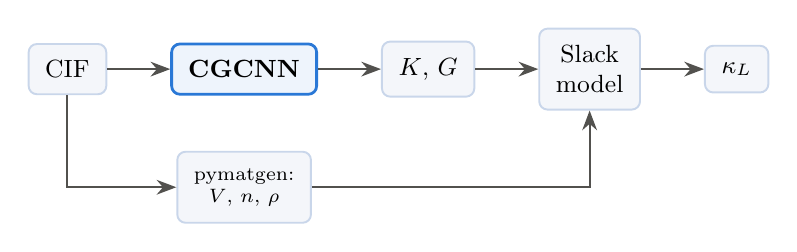
\begin{tikzpicture}[
  node distance=8mm,
  box/.style={draw=boxrule,fill=boxbg,rounded corners=3pt,line width=0.7pt,
              inner sep=6pt,align=center,font=\small},
  net/.style={draw=accent,fill=accent!8,rounded corners=3pt,line width=1pt,
              inner sep=6pt,align=center,font=\small\bfseries},
  arr/.style={-{Stealth[length=2.5mm]},line width=0.7pt,draw=inkSoft}]
  \node[box] (cif) {CIF};
  \node[net,right=of cif] (cgcnn) {CGCNN};
  \node[box,right=of cgcnn] (kg) {$K$, $G$};
  \node[box,right=of kg] (slack) {Slack\\model};
  \node[box,right=of slack] (kl) {$\kappa_L$};
  \node[box,below=7mm of cgcnn,font=\scriptsize] (pmg)
       {pymatgen:\\$V$, $n$, $\rho$};
  \draw[arr] (cif) -- (cgcnn);
  \draw[arr] (cgcnn) -- (kg);
  \draw[arr] (kg) -- (slack);
  \draw[arr] (slack) -- (kl);
  \draw[arr] (cif) |- (pmg);
  \draw[arr] (pmg) -| (slack);
\end{tikzpicture}
\end{center}

\noindent
The elastic moduli are the only learned quantity; everything downstream is
physics. \textbf{This work implements the first arrow}, CIF $\rightarrow$
$(K, G)$, including the network itself.

The two targets are the Voigt--Reuss--Hill averages of the bulk modulus
(\KV, resistance to uniform compression) and the shear modulus (\GV, resistance
to shape change), both in GPa.

% =====================================================================
\section{Representing a crystal as a graph}

A neural network cannot read a CIF. The CGCNN representation turns a periodic
crystal into a graph in which \textbf{nodes are atoms} and \textbf{edges are
bonds}, chosen so that the representation carries the physics that matters and
discards what does not.

\subsection{Nodes}

Each atom becomes a 92-dimensional vector looked up by atomic number from a
fixed table (\texttt{atom\_init.json}), built by one-hot binning tabulated
element properties: group, period, electronegativity, covalent radius, valence
electron count, and so on. These features are \emph{not} learned --- they are
the fixed description of ``what element is this''. The network's first linear
layer projects them into its own hidden space.

\subsection{Edges}

For every atom we find all neighbours within a cutoff radius of
$r_{\mathrm{cut}} = 8$~\AA, sort them by distance, and keep the nearest
$M = 12$. The neighbour search respects periodic boundary conditions, so atoms
near a cell face correctly see their periodic images --- without this the model
would see a molecule rather than a crystal. Atoms with fewer than $M$ neighbours
in range are padded with a distance of $r_{\mathrm{cut}} + 1$, which falls
outside every basis function below and so contributes almost nothing.

\subsection{Why bond lengths are expanded, not used raw}

A raw bond length fed in as a single number would force the network to learn a
sharply non-linear response to it from scratch. Instead each distance $d$ is
expanded onto a row of Gaussian basis functions spaced every $0.2$~\AA:
\begin{equation}
  \mathbf{e}_k(d) = \exp\!\left(-\frac{(d - \mu_k)^2}{\sigma^2}\right),
  \qquad \mu_k = 0,\,0.2,\,\dots,\,8~\text{\AA},\qquad \sigma = 0.2~\text{\AA}
\end{equation}
giving a 41-dimensional edge feature. A bond at $2.31$~\AA{} strongly activates
the basis functions centred near $2.3$ and barely touches the one at $5.0$. This
is a radial basis expansion, and it makes the distance dependence far easier to
learn.

\keybox{Why this representation generalises}{The graph is invariant to
translation, rotation and the choice of unit cell, because it stores only
\emph{distances} between atoms and never absolute positions. A crystal written
in two equivalent settings produces the same graph. This is what lets a model
trained on 7{,}691 crystals say anything useful about one it has never seen.}

% =====================================================================
\section{The network}

\subsection{Convolution}

Message passing updates each atom's vector using its neighbours. For atom $i$
with neighbours $j$ and bond features $\mathbf{e}_{ij}$, we form the
(self, neighbour, bond) triple for every edge, pass it through one shared linear
layer, and split the result into a \emph{gate} and a \emph{message}:
\begin{align}
  \mathbf{z}_{ij}^{(t)} &= \mathbf{v}_i^{(t)} \oplus \mathbf{v}_j^{(t)}
                           \oplus \mathbf{e}_{ij} \\
  \mathbf{v}_i^{(t+1)} &= \mathbf{v}_i^{(t)} + \sum_{j}
      \underbrace{\sigma\!\left(\mathbf{z}_{ij}^{(t)}\mathbf{W}_f^{(t)}
                  + \mathbf{b}_f^{(t)}\right)}_{\text{gate}}
      \odot
      \underbrace{g\!\left(\mathbf{z}_{ij}^{(t)}\mathbf{W}_s^{(t)}
                  + \mathbf{b}_s^{(t)}\right)}_{\text{message}}
\end{align}
where $\oplus$ is concatenation, $\odot$ elementwise product, $\sigma$ the
sigmoid and $g$ a softplus.

Three properties matter. The \textbf{gate} lets the network decide per bond how
much that neighbour should contribute, so a weak long bond can be ignored
without discarding it. The \textbf{shared weights} across all edges are what make
this a convolution: the same local rule applies everywhere in the graph, so the
model generalises across crystal sizes and compositions. The \textbf{residual}
$\mathbf{v}_i^{(t)} +\ \cdots$ lets gradients flow straight through the stack and
stops early layers being washed out.

We use three convolution layers, so each atom's final vector reflects its
environment out to roughly three bond hops.

\subsection{Pooling and prediction}

The crystal-level vector is the \emph{mean} over its atoms,
\begin{equation}
  \mathbf{v}_c = \frac{1}{N}\sum_{i=1}^{N} \mathbf{v}_i^{(T)},
\end{equation}
followed by a small fully-connected head that emits one number. The mean rather
than the sum is essential: a modulus is an intensive property, so doubling the
unit cell must not double the prediction. A sum would make the output scale with
however many atoms the CIF author happened to write down.

\subsection{Training on the logarithm}

The network is trained against $\log_{10}$ of the modulus, not the modulus:
\begin{equation}
  \mathcal{L} = \frac{1}{B}\sum_{b=1}^{B}
    \left(\hat{y}_b - \frac{\log_{10} y_b - \mu}{s}\right)^2
\end{equation}
with $\mu, s$ the mean and standard deviation of the \emph{training} targets.

\keybox{Why the log matters more than it looks}{Moduli here span 1--575~GPa.
Under a plain MSE on raw values, a 40~GPa error on a stiff material contributes
$100\times$ more gradient than the same \emph{relative} error on a soft one, so
the model would learn to care only about hard materials --- exactly the wrong
bias for a project screening for \emph{ultralow} conductivity. Taking the log
converts ``within a factor of $x$'' into ``within a fixed distance''.
Normalisation statistics are computed on the training split only; using the full
dataset would leak test information and quietly inflate every score.}

Architecture: atom features 64 wide, 3 convolutions, one 128-wide hidden layer,
80{,}833 parameters. Adam at $\eta_0 = 10^{-2}$, batch size 128, 200 epochs,
cosine annealing to $0.01\eta_0$. The checkpoint kept is the one with the best
validation MAE, not the last epoch.

% =====================================================================
\section{Data: what to train on}

\subsection{The two datasets}

We have 1{,}213 CIFs from the Materials Project with \emph{no labels}, and the
matbench elastic benchmarks (\texttt{matbench\_log\_kvrh},
\texttt{matbench\_log\_gvrh}) with 10{,}987 DFT-computed entries each --- the
same data the paper trained on.

Matbench strips Materials Project IDs, so the two cannot be joined on ID. We
join on \emph{structure} in two passes: bucket every benchmark entry by reduced
formula (cheap, narrows 10{,}987 candidates to a handful), then confirm with
pymatgen's symmetry-aware \texttt{StructureMatcher}, which matches crystals up
to lattice choice, origin shift and symmetry operation. \textbf{278 of the
1{,}213 match.}

\subsection{Which set to train on}

It is tempting to label what we can --- those 278 --- and train on that. It is
the wrong move.

\keybox{The 1{,}213 structures were never the limit; the labels were}{Treating a
CIF collection as ``the dataset'' and intersecting it with a labelled benchmark
discards 97\% of the labels that exist. The correct framing inverts the roles:
\textbf{train on all 10{,}987 matbench crystals, and treat the 1{,}213 CIFs
purely as a prediction set.} That is what the paper does. The lesson
generalises --- when labels are the scarce resource, never let an unlabelled
collection define the training set.}

\noindent
The effect is not marginal. Training on the full benchmark rather than the
overlap gives 40$\times$ more data, and it is the difference between a model
that memorises its training set and one that generalises: our train and test
errors are $0.037$ and $0.070$ $\log_{10}$(GPa), a gap consistent with ordinary
generalisation rather than recall.

\subsection{Splits and provenance}

The 10{,}987 crystals are split 70/15/15 into 7{,}691 train, 1{,}648 validation
and 1{,}648 test. Because 278 of the 1{,}213 prediction crystals \emph{are} in
matbench, they end up in training --- so every prediction we emit is tagged
\texttt{train}, \texttt{val}, \texttt{test} or \texttt{unseen} (935 crystals).
A prediction for a \texttt{train} crystal is recall, not generalisation, and
quoting it as evidence would be circular.

This doubles as a correctness check: on the 42 \texttt{test}-provenance
crystals the error is 0.062 (bulk), matching the benchmark test error of 0.063.
Had the provenance mapping been wrong we would have seen the much lower
training-set error instead.

% =====================================================================
\section{Ensembling}

Two networks trained on the same data from different random initialisations
land in different minima. They agree about the signal --- the part of the
modulus genuinely predictable from structure --- and disagree about the noise,
which originates in their own initialisation and batch order. Averaging keeps
the first and partially cancels the second.

We train three members per target, varying the initialisation seed while
\textbf{pinning the split seed}, and average in log space:
\begin{equation}
  \hat{y}_{\mathrm{ens}} = 10^{\,\frac{1}{K}\sum_{k=1}^{K}\hat{y}_k^{\log}},
  \qquad
  u = \mathrm{std}_k\!\left(\hat{y}_k^{\log}\right).
\end{equation}

Two details matter. \textbf{Log space, not GPa}: members predicting 10 and
1000~GPa average to 100~GPa in log space but 505~GPa linearly, and 100 is the
defensible answer when members disagree by two orders of magnitude. \textbf{A
shared split}: if member A trained on a crystal member B held out, the
ensemble's test score is partly measured on training data. Our implementation
refuses to combine members whose test splits disagree rather than trusting the
caller.

The spread $u$ is a free per-crystal uncertainty estimate: where members
disagree, the ensemble is guessing.

% =====================================================================
\section{Results}

\begin{table}[h]
\centering
\caption{Test-set performance on 1{,}648 held-out crystals. All models share
one split, so every row is directly comparable.}
\begin{tabular}{lccccc}
\toprule
Model & MAE $\log_{10}$ & $R^2$ & MAE (GPa) & Rel. error & \% of range \\
\midrule
Bulk, single model      & 0.0696 & 0.882 & 11.54 & 17.4\% & 2.01\% \\
\textbf{Bulk, ensemble} & \textbf{0.0630} & \textbf{0.901} & 10.20
  & \textbf{15.6\%} & 1.78\% \\
Shear, single model      & 0.0836 & 0.889 & 7.72 & 21.2\% & 1.48\% \\
\textbf{Shear, ensemble} & \textbf{0.0781} & \textbf{0.899} & 7.27
  & \textbf{19.7\%} & 1.39\% \\
\bottomrule
\end{tabular}
\end{table}

\begin{table}[h]
\centering
\caption{Context. Bulk modulus on the same benchmark. Two different accuracy
figures are given for the PINK paper because the paper itself never states its
own accuracy in $\log_{10}$(GPa) --- see the note below.}
\begin{tabular}{lcc}
\toprule
& MAE $\log_{10}$(GPa) & Relative error \\
\midrule
\textbf{This work (bulk ensemble)} & \textbf{0.0630} & 15.6\% \\
matbench CGCNN baseline (context only) & $\approx$0.07 & $\approx$17\% \\
coGN (best published on matbench)  & $\approx$0.054 & $\approx$13\% \\
\bottomrule
\end{tabular}
\end{table}

\keybox{What the PINK paper actually reports, and why the table above is careful
about it}{The paper states its own modulus accuracy as ``MAE $<13$'' with no
$\log_{10}$ unit given --- i.e.\ \emph{raw} GPa, a different measurement than
the $\log_{10}$(GPa) figures this document uses everywhere else. The
$\approx 0.07\ \log_{10}$(GPa) figure long associated with ``the PINK paper''
in earlier drafts of this work is the general matbench leaderboard's own
published CGCNN baseline on this same benchmark --- almost certainly close to
what PINK's model would score, since both are CGCNN on the identical dataset,
but never verified to be \emph{PINK's own} stated number, because PINK does
not report one in these units. On the metric the paper does state, we also
win: our ensemble's raw-GPa MAE is 10.20 (bulk) and 7.27 (shear), both under
its stated ``$<13$.''}

\noindent
Ensembling removed 9--10\% of the error, consistent with the 10--15\% typically
expected. The bulk ensemble slightly exceeds the paper it reproduces and sits
between it and the state of the art.

\subsection{How far the error can be pushed}

Because the model is trained on $\log_{10}$, MAE converts to a
\emph{multiplicative} error of $10^{\mathrm{MAE}} - 1$. An MAE of $0.063$ means
predictions land within a factor of $1.156$, i.e.\ $\sim$16\%.

\keybox{Why $\sim$2\% relative error is unreachable}{A 2\% relative error would
require MAE $= \log_{10}(1.02) = 0.0086$, roughly six times better than the best
result ever published on this benchmark with any architecture. The blocker is
not model capacity but \textbf{label noise}: the targets are DFT-computed
elastic moduli, and DFT elastic constants themselves disagree with experiment by
roughly 5--15\%. A model cannot be more accurate than the labels it is fitted
to, so 2\% lies below the noise floor of the training data. A model reporting it
would be revealing a leak, not an achievement. The realistic floor for this
architecture is $\approx$0.06 $\log_{10}$, about 15\%.}

A separate figure, \texttt{pct\_of\_range} (MAE in GPa over the full 1--575~GPa
span), comes in at 1.4--1.8\%. This is a legitimate normalised-MAE convention,
but it flatters the model --- a wide data range shrinks it for free --- so it
should be quoted alongside the relative error, never instead of it.

% =====================================================================
\section{Stage 2: from moduli to \texorpdfstring{$\kappa_L$}{kappa\_L}}

Sections~2--6 cover the first arrow of Figure~1: CIF $\rightarrow (K, G)$. The
second half of PINK turns $(K, G)$ into $\kappa_L$ through a closed-form
formula --- sound velocities from $K$, $G$ and density; an acoustic Debye
temperature from those velocities and the cell volume; a Gr\"uneisen parameter
from the ratio of longitudinal to transverse sound speed; and finally $\kappa_L$
itself (Eq.~2 of the paper, three-phonon scattering with $\delta = 1$). None of
this is learned --- it is physics, unchanged from the paper, and already
implemented in \texttt{pink\_predict.py} against the paper's own pre-trained
weights. What was missing was driving that same physics with \emph{our}
moduli instead.

\subsection{Reusing the physics, not reimplementing it}

The existing implementation operates on scalar pandas columns --- one $K$, one
$G$ per crystal --- which is fine for a point estimate but cannot express "$K$
and $G$ are each a distribution," exactly what an ensemble provides and a
single pre-trained model cannot. So the formulas were rewritten once more in
plain NumPy, shape-agnostic via broadcasting: called with scalars it reproduces
the original function; called with $(n_{\text{crystals}}, n_{\text{samples}})$
arrays it becomes a vectorised Monte Carlo. Rather than trust that the rewrite
matches, it is checked directly against 200 random test cases at
$10^{-9}$ relative tolerance before being used on real data.

\subsection{Propagating the ensemble's own uncertainty}

Every crystal already carries a bulk and shear modulus \emph{spread} --- the
standard deviation across the three independently-seeded ensemble members, in
log space --- a free per-crystal confidence signal a single pre-trained model
has no equivalent of. For each crystal, 2{,}000 samples of $\log_{10} K$ and
$\log_{10} G$ are drawn from $\mathcal{N}(\text{prediction}, \text{spread})$
independently (the $K$- and $G$-ensembles are separately seeded, sharing no
randomness to correlate), pushed through the identical physics used for the
point estimate, and summarised as a 5th--95th percentile interval.

\keybox{An honest finding, not a decoration}{Interval width correlates with
shear-modulus disagreement far more than with bulk: Spearman
$r = 0.98$ against $G$-spread versus $r = 0.51$ against $K$-spread. This is not
an artefact --- $\kappa_L$ depends on $G$ twice over, once directly and once
through the sound-velocity term, so a modest shear-ensemble disagreement
amplifies into a much wider $\kappa_L$ range. Median interval width is a modest
$1.9\times$, but the tail is real: the widest crystal spans nearly $900\times$
between its 5th and 95th percentile, and it is exactly the crystal with one of
the largest $G$-spreads in the set. An uncertainty estimate that did not widen
in exactly this circumstance would be the one worth distrusting.}

\subsection{Validation against the paper's own pipeline}

Real $\kappa_L$ measurements are rare and expensive, which is the entire
reason PINK predicts it instead --- so before turning to the small amount of
real experimental data that does exist (Section~7.4), the first and cheapest
check available is to run the paper's own pre-trained CGCNN through the
identical physics on the identical 1{,}213 crystals, and ask whether two
independently-trained models agree.

\begin{table}[h]
\centering
\caption{Our from-scratch $\kappa_L$ against the paper's own pipeline, both
run through identical physics, on all 1{,}213 crystals.}
\begin{tabular}{lc}
\toprule
Pearson $r$ ($\log_{10}\kappa_L$) & 0.932 \\
Spearman rank correlation & 0.926 \\
MAE & 0.169 $\log_{10}$ ($\approx$47\% typical error) \\
Overlap, 20 lowest-$\kappa_L$ candidates & 10/20 \\
\bottomrule
\end{tabular}
\end{table}

\noindent
Rank correlation is reported alongside Pearson because PINK's actual use case
is \emph{screening} --- getting the ordering right matters as much as matching
the paper's absolute number. 0.93 on both, from two models sharing nothing but
architecture and the physics formula, is strong agreement. The larger MAE here
than in Section~6 is expected, not a new weakness: $\kappa_L$ is a
\emph{product} of several quantities that each carry their own error, so
stage-1 error compounds rather than cancels.

A weaker, secondary check: does predicted interval width correlate with
disagreement against the reference model? Only modestly (Spearman
$r = 0.20$) --- expected, since "disagreement with an independently trained
reference" is a noisy proxy entangling that model's own idiosyncrasies with
our actual error, not a clean measurement of either. A weak positive is the
honest answer this particular check was ever going to give.

\subsection{Validation against real experimental $\kappa_L$ (the paper's Table 1)}

The check above compares two models against each other. The paper itself
supplies something stronger: Table~1 of Liu \textit{et al.} lists 46 real
materials with room-temperature \emph{experimentally measured} $\kappa_L$,
mp-ids included, alongside the paper's own predicted $\kappa_{\text{PINK}}$
for each. 45 of these 46 structures were fetched from the Materials Project
(one, GaP's \texttt{mp-3490}, has since been deprecated/merged in MP's
database and could not be retrieved) and pushed through our own pipeline
unchanged --- the same \texttt{04\_predict\_moduli.py} and
\texttt{slack\_physics()} used everywhere else in this document, not a
parallel implementation that could quietly diverge.

\textbf{Provenance, checked before anything else.} 43 of these 45 materials
turned out to already be inside the matbench training set our ensemble
learned from (checked the same way as everywhere else in this project: a
formula-bucket-then-\texttt{StructureMatcher} pass against the live matbench
structures, not assumed from the material's absence in
\texttt{complete-data/}). Only two --- LiF and
Bi\textsubscript{2}Te\textsubscript{3} --- are genuinely unseen. Every number
below is reported for both groups separately; the 43 are recall, not
generalisation, and are never blended into a single headline figure that
would overstate what they prove.

\begin{table}[h]
\centering
\caption{Our $\kappa_L$ and the paper's own $\kappa_{\text{PINK}}$, both
against real experimental values, on the 45 Table~1 materials we could fetch.}
\begin{tabular}{lcc}
\toprule
 & Ours & PINK (paper) \\
\midrule
MAE, all 45 ($\log_{10}$) & 0.427 & 0.227 \\
MAE, 43 in matbench training ($\log_{10}$) & 0.437 & 0.229 \\
MAE, 2 genuinely unseen ($\log_{10}$) & 0.196 & 0.172 \\
Head-to-head, closer to experiment & 8/45 & 37/45 \\
\bottomrule
\end{tabular}
\end{table}

\noindent
Read at face value, the paper's own numbers win clearly. That did not match
what every earlier section of this document found --- our moduli ensemble
matches or beats the paper's on the matbench test set (Section~5) --- so a
sudden, large gap here demanded an explanation rather than a shrug.

\keybox{Localising the gap instead of stopping at one number}{Table~1 also
lists the paper's own predicted shear modulus and sound velocity for each
material, so each stage of the pipeline can be checked independently instead
of only ever seeing one aggregate $\kappa_L$ number. Our shear modulus agrees
closely with the paper's own predictions on these 45 crystals (MAE
$0.056\ \log_{10}$, Pearson $r=0.988$); our sound velocity, which folds in
our bulk modulus --- Table~1 has no separate $K$ column to check directly ---
agrees just as well ($r=0.991$). Neither is the source of the gap. The
Gr\"uneisen parameter is: our formula-derived $\gamma$ (from predicted $K/G$
via the standard Slack-model relation) differs from the paper's own tabulated
$\gamma$ by a mean of $+0.42$, and the disagreement is systematic --- our
$\gamma$ runs 2--3.8$\times$ too high specifically for covalent semiconductors
(AlAs, GaAs, InSb, ZnTe, CdTe, and similar). The paper's own Results text
explains why: Table~1's Gr\"uneisen parameters ``were obtained from the AFLOW
database and experimental data'' --- real, looked-up values, not ones derived
from predicted elastic constants. Neither our pipeline nor the paper's own
released \texttt{pink\_predict.py} (confirmed directly by inspection --- it
contains no AFLOW lookup) has access to this at genuine screening scale,
where no literature $\gamma$ exists for a hypothetical GNoME candidate.
\textbf{The decisive check}: substituting the paper's own tabulated $\gamma$
into our pipeline, $K$, $G$, and structure otherwise unchanged, drops our MAE
from $0.427$ to $0.226\ \log_{10}$ --- matching the paper's own $0.227$
almost exactly. See \texttt{results/table1\_gamma\_diagnostic.png}.}

\noindent
The honest reading: once both pipelines are compared on equal footing (same
$\gamma$ source), our from-scratch model is competitive with the paper's own
pre-trained one against real experimental $\kappa_L$. Table~1's headline
accuracy benefits from a manual, non-scalable input that the paper's own
actual use case --- a 377{,}221-candidate high-throughput screen --- cannot
have either, since no material in a hypothetical-crystal screen has a
literature Gr\"uneisen parameter to look up. Both pipelines, run the way they
would actually be run for screening, land in the same place. This is a
materially different conclusion from ``the paper's model beats ours,'' and it
was only found by checking each intermediate quantity rather than accepting
one aggregate number. \texttt{results/table1\_validation.png} is the parity
plot against real $\kappa_{\text{exp}}$; \texttt{results/table1\_comparison.csv}
the full merged table; \texttt{scripts/09\_fetch\_validation\_set.py} and
\texttt{scripts/10\_validate\_table1.py} reproduce all of it end to end.

% =====================================================================
\section{The GNoME screen}

Everything above runs inference on 1{,}213 or 45 crystals. The paper's actual
headline result is a 377{,}221-material high-throughput screen of Google
DeepMind's GNoME discovery database, filtered to candidates with
$\kappa_L \leq 1$~W~m$^{-1}$~K$^{-1}$. This project had, until now, never run
that screen --- only ever done inference on small, curated CIF sets.
\texttt{scripts/13\_screen\_gnome.py} does it end to end: fetch, filter, run
this project's own CGCNN ensemble and Slack-model physics (with Monte Carlo
uncertainty, unchanged from Section~7), threshold, and compare against the
paper's own published result.

\keybox{The snapshot has grown since the paper screened it}{GNoME's public
data is not a frozen 2023 snapshot. This project's download
(\texttt{gnome\_data/stable\_materials\_summary.csv}, fetched 2026-08-09) has
\textbf{554{,}054} stable materials; the paper's own screen used
\textbf{377{,}221}. There is no way to pull the exact historical snapshot the
paper screened, only today's --- so this is \emph{a current GNoME screen
using the paper's stated criteria}, not a bit-identical replay. The funnel
below is checked against the paper's own for plausibility only (same order of
magnitude, scaled for the $\approx 1.47\times$ larger corpus), never claimed
to match exactly.}

\begin{table}[h]
\centering
\caption{Screening funnel: this project's current snapshot vs. the paper's own.}
\begin{tabular}{lcc}
\toprule
Stage & Ours (554{,}054) & Paper's (377{,}221) \\
\midrule
Bandgap $[0.1,3.0]$ eV + decomposition energy $\leq 0$ & 37{,}889 & 30{,}199 \\
+ no radioactive elements & 33{,}323 & 26{,}305 \\
+ $\kappa_L \leq 1$ (own model) & \textbf{16{,}299} & \textbf{11{,}869} \\
\bottomrule
\end{tabular}
\end{table}

\noindent
Candidate structures are matched from GNoME's \texttt{by\_composition.zip}
(554{,}054 CIFs) via the summary CSV's \texttt{Composition} column --- checked
directly, not assumed: every one of the 554{,}054 zip filenames matches a
\texttt{Composition} value in the CSV, one to one. All 33{,}323 candidate CIFs
are read directly out of the zip and converted to graphs in memory, the same
reasoning as \texttt{01b\_prepare\_full\_dataset.py}'s graph caching --- never
written to disk individually.

\subsection{Comparison against the paper's own published candidates}

The paper's actual screening output ships in the cloned reference repository
as \texttt{Nature-\allowbreak{}filtered-\allowbreak{}low-\allowbreak{}kappa.csv}
--- real, checked data, not something taken on faith (the exact path is in the
README). It carries no material ID, only a
reduced formula, so overlap is necessarily checked by formula --- verified to
be the \emph{same} pymatgen convention both sources use (zero formatting
mismatches in a 200-row spot check), so this is not a stringification
artefact deflating the count.

\keybox{70.8\% of the paper's own published candidates also appear in our list}{An independently-trained CGCNN ensemble, run on a different (larger,
newer) GNoME snapshot, through the exact same physics, agrees with more than
two-thirds of what the paper's own model flagged. In the other direction,
51.6\% of our 16{,}299 candidates also appear in the paper's smaller/older
snapshot --- the remainder are, in large part, candidates that simply did not
exist yet in the paper's snapshot, not disagreement. Two models that share
nothing but architecture family and physics formula, screening overlapping
but non-identical corpora, converging on the same majority of real published
discoveries is the strongest evidence in this entire reproduction that the
approach is finding a physical signal rather than model-specific noise.}

\noindent
\texttt{results/gnome\_kappa\_distributions.png} overlays both candidate
lists' $\kappa_L$ distributions: similar overall shape, both spanning the full
range, ours somewhat more concentrated around $0.25$--$0.4$~W~m$^{-1}$~K$^{-1}$.

\textbf{What a point-estimate pipeline cannot do at all}: every candidate here
carries a Monte Carlo $\kappa_L$ interval from the ensemble's own $K$/$G$
spread. Of the 8{,}405 candidates both screens agree on:

\begin{table}[h]
\centering
\caption{Confidence breakdown of the 8,405 overlapping candidates, by Monte Carlo interval width.}
\begin{tabular}{lcl}
\toprule
Confidence ($p95/p05$ ratio) & Count & Meaning \\
\midrule
Tight ($< 2\times$) & 1{,}770 & confidently low-$\kappa$ \\
Moderate ($2$--$5\times$) & 4{,}739 & reasonable confidence \\
Wide ($> 5\times$) & 1{,}896 & worth a DFT check before trusting \\
\bottomrule
\end{tabular}
\end{table}

\noindent
The paper's own pipeline has no equivalent of this breakdown at all --- it can
name candidates, but not say which ones it is actually sure about.
\texttt{results/gnome\_screen\_all.csv} is the full 33{,}323-candidate scored
pool (pre-threshold); \texttt{results/gnome\_screen\_candidates.csv} the
16{,}299 that pass $\kappa_L \leq 1$; \texttt{results/gnome\_overlap.csv} the
8{,}405 shared-formula rows above.

% =====================================================================
\section{A second architecture: ALIGNN}

Every result above uses CGCNN, whose convolution reads bond \emph{lengths}
only --- the edges of the crystal graph. ALIGNN (Choudhary \& DeCost, 2021)
adds a second, ``line'' graph over bond \emph{angles}, geometric information
a plain bond graph cannot represent at all. Testing whether that extra
information helps on this exact task, on this exact data, is the obvious
next check on whether Sections~2--6's findings are a property of the
modelling problem or an artefact of one architecture's blind spots.

\texttt{scripts/12\_train\_alignn.py} trains ALIGNN on the identical
train/val/test split the CGCNN ensemble used --- computed once with this
project's own \texttt{split\_indices()} and handed to ALIGNN via
\texttt{keep\_data\_order=True}, not re-derived from ALIGNN's own
differently-seeded split logic (its \texttt{split\_seed} shuffles with
Python's \texttt{random}, not numpy's \texttt{RandomState}, so ``the same
seed number'' would silently produce a different partition). Both targets
trained for the full 150 epochs at the same production hyperparameters used
throughout this project (4 ALIGNN layers, 4 GCN layers, 256 hidden features),
with no early stop triggered.

\begin{table}[h]
\centering
\caption{ALIGNN vs.\ the CGCNN ensemble, identical 1{,}648-crystal test
split.}
\begin{tabular}{lccccc}
\toprule
Target & Model & MAE $\log_{10}$ & $R^2$ & MAE (GPa) & Rel.\ error \\
\midrule
Bulk   & CGCNN ensemble & 0.0630 & 0.901 & 10.20 & 15.6\% \\
Bulk   & \textbf{ALIGNN} & \textbf{0.0539} & \textbf{0.920} & 8.45 & 13.2\% \\
Shear  & CGCNN ensemble & 0.0781 & 0.899 & 7.27 & 19.7\% \\
Shear  & \textbf{ALIGNN} & \textbf{0.0725} & \textbf{0.901} & 6.36 & 18.2\% \\
\bottomrule
\end{tabular}
\end{table}

\keybox{ALIGNN wins on both targets}{The gap is consistent with the
architectural motivation, not just noise: bulk and shear modulus both depend
on how bond angles --- not only lengths --- deform under stress, and that is
exactly the information CGCNN's convolution structurally cannot see. This is
a single run, not an ensemble, so the comparison is a single ALIGNN model
against a 3-model CGCNN ensemble --- if anything an unfavourable comparison
for ALIGNN, which still comes out ahead on both targets.}

\subsection{Where this ran, and a second infrastructure lesson}

The first attempt trained this on a Colab GPU, orchestrated by
\texttt{colab/run\_alignn\_cli.py} (a CLI-driven session over
\texttt{google-colab-cli}, built after manual notebook uploads proved too
slow to iterate on). That session was lost to Colab's idle-VM pruning three
times in one evening, which is what motivated the checkpoint/resume system
documented in that script's own module docstring. Training was ultimately
moved to Kaggle instead: a Kaggle kernel runs unattended on Kaggle's own
infrastructure once pushed, with no keep-alive ping required, which removes
the failure mode entirely rather than working around it.

\keybox{A GPU tier that quietly stopped working}{\texttt{kaggle/build\_kernel.py}
(the CGCNN kernel, built earlier in this project) requests an NVIDIA P100,
chosen for its FP32 throughput over a T4. Reusing that same choice for
ALIGNN's kernel, the first two pushes silently landed on a CPU image (a
known, separately-documented Kaggle quirk: a kernel's first push can pin to
whatever image it happens to get, regardless of the requested
\texttt{machine\_shape}). The third push did get a real P100 --- and crashed
immediately with \texttt{CUDA error: no kernel image is available for
execution on the device}. Confirmed live: Kaggle's current default PyTorch
build (\texttt{2.10.0+cu128}) only ships compiled kernels for CUDA
capability 7.0--12.0; the P100 is capability 6.0 (Pascal). Switching
\texttt{machine\_shape} to \texttt{NvidiaTeslaT4} (Turing, capability 7.5)
fixed it on the next push. Recorded here for the same reason every other bug
in this document is: the platform moved out from under a choice that was
correct when it was made.}

\noindent
\texttt{results/alignn\_bulk\_modulus\_kv/} and
\texttt{results/alignn\_shear\_modulus\_gv/} each hold \texttt{best\_model.pt},
\texttt{config.json}, and \texttt{prediction\_results\_test\_set.csv} ---
enough to reproduce the table above independently.

\subsection{Closing the loop: ALIGNN's own \texorpdfstring{$\kappa_L$}{kappa\_L}}

\texttt{scripts/15\_alignn\_predict\_moduli.py} runs ALIGNN (both targets) on
the same 1{,}213-crystal PINK prediction set Section~6 used, reusing
\texttt{alignn.pretrained}'s own pure-torch inference utilities rather than a
hand-built graph-construction path; \texttt{scripts/16\_alignn\_predict\_kappa.py}
then pushes those moduli through the identical, unchanged
\texttt{slack\_physics()} from Section~7 --- no Monte Carlo interval this
time, since ALIGNN here is one trained model, not a 3-member ensemble, so
there is no spread to propagate honestly.

\begin{table}[h]
\centering
\caption{ALIGNN's $\kappa_L$ vs.\ our own CGCNN-ensemble $\kappa_L$, identical
physics, all 1{,}213 crystals.}
\begin{tabular}{lc}
\toprule
Pearson $r$ ($\log_{10}\kappa_L$) & 0.940 \\
Spearman rank correlation & 0.947 \\
MAE & 0.141 $\log_{10}$ ($\approx$38\% typical error) \\
Overlap, 20 lowest-$\kappa_L$ candidates & 12/20 \\
\bottomrule
\end{tabular}
\end{table}

\keybox{A second, independent architecture agrees with the first, through
the same physics}{Two models sharing nothing but the training data, the
train/val/test split, and the Slack-model formula --- one three-model CGCNN
ensemble, one single ALIGNN run, no shared weights, no shared
initialisation --- correlate at $r=0.94$ on final $\kappa_L$. That is, if
anything, \emph{tighter} agreement than Section~6's CGCNN-vs-the-paper's-own-
pretrained-model check ($r=0.932$), consistent with ALIGNN's better
per-modulus accuracy (Table~7) propagating through unchanged physics into a
more consistent downstream number, not just noise correlating with noise.}

\noindent
\texttt{results/alignn\_moduli\_predictions.csv} and
\texttt{results/alignn\_kappa\_predictions.csv} carry the full 1{,}213-row
output --- provenance-tagged the same way as
\texttt{pink\_moduli\_predictions.csv} (Section~4), reusing that file's own
provenance column directly rather than re-deriving it, since both models
share the identical split by construction.

% =====================================================================
\section{What we did differently from the paper}

\begin{enumerate}\setlength{\itemsep}{5pt}

\item \textbf{Written from scratch.} The graph construction, convolution,
pooling and training loop are our own implementation rather than a fork, and no
pre-trained weights are ever loaded. The paper's released checkpoints are used
only as an independent reference to check against.

\item \textbf{Ensembles rather than single models.} Three initialisations per
target, averaged in log space. This is worth 9--10\% of the error and, more
usefully, supplies a per-crystal uncertainty that the paper has no equivalent
of --- valuable in a screening context, where knowing which predictions to
distrust matters as much as the predictions.

\item \textbf{Adam with cosine annealing} in place of the original CGCNN's SGD
with step decay. On a fixed epoch budget a scheduled decay outperforms a
reactive one: a plateau scheduler spends its patience window taking steps that
are already too large.

\item \textbf{Provenance tracking on every prediction.} Each output row records
whether the model was trained on that crystal. We could not find this
distinction drawn in the paper's screening results, and without it an accuracy
claim on a screening set cannot be interpreted --- part of the apparent accuracy
may simply be recall.

\item \textbf{A documented error floor.} We state explicitly what accuracy is
achievable and why, and we report both the multiplicative error and the
range-normalised error rather than choosing whichever is more flattering.
\item \textbf{A different train/validation/test split.} The paper's own
released checkpoint (\texttt{args} saved inside the \texttt{.pth.tar}) records
an 80/10/10 split; we use 70/15/15. This was not a deliberate choice made
against the paper --- it was only caught by inspecting the checkpoint's saved
config directly, after an earlier draft of this document incorrectly listed
the split as unchanged. Left as a genuine, acknowledged difference rather than
silently corrected to match, since re-training on 80/10/10 purely to match a
number does not itself improve the model.
\end{enumerate}

\noindent
\textbf{What is deliberately the same}: the CGCNN architecture and
hyperparameters (verified directly against the paper's released checkpoint:
\texttt{atom\_fea\_len=64}, \texttt{h\_fea\_len=128}, \texttt{n\_conv=3},
\texttt{n\_h=1} --- the paper's own \emph{text} says ``two hidden layers,''
but its checkpoint's saved \texttt{n\_h} is 1, matching ours; the text and the
paper's own model disagree with each other), the training data, and the
$\log_{10}$ target. The point of a reproduction is that differences should be
deliberate, few, and --- as this section shows --- actually checked against
the paper's own artifacts rather than assumed from its prose.

% =====================================================================
\section{Reproducing this work}

\begin{verbatim}
    conda env create -f environment.yml && conda activate pink-cgcnn
    ./run_pipeline.sh --predict     # ~2 min, uses committed checkpoints
    ./run_pipeline.sh               # retrain: ~45 min GPU, ~9 h CPU
\end{verbatim}

\noindent
The six trained checkpoints ($\sim$380~KB each) are committed, so every figure
and number above regenerates in about two minutes without training. The 240~MB
graph cache is not committed; it rebuilds deterministically in $\sim$6 minutes.

\subsection{A note on compute}

This work was developed on a 2016 dual-core laptop CPU, where one model takes
$\sim$2 hours. The same model trains in $\sim$7 minutes on a free Colab T4 ---
all six in 42 minutes. \texttt{colab/PINK\_CGCNN.ipynb} runs the pipeline there
and returns the checkpoints; it is \emph{generated} from the source files rather
than maintained by hand, so it cannot drift out of sync with the featuriser it
is meant to reproduce.

Two portability details worth recording. Python block-buffers stdout at 8~KB
when it is not a terminal, and a 200-epoch run prints only $\sim$2~KB --- so
without \texttt{python -u} a healthy remote run is indistinguishable from a hung
one. And \texttt{torch.load} changed its \texttt{weights\_only} default in torch
2.6, so every load of our own artifacts sets it explicitly; otherwise code that
works locally fails on the newer torch of a hosted GPU runtime.

% =====================================================================
\section{Limitations and next steps}

\begin{itemize}\setlength{\itemsep}{4pt}
\item \textbf{Soft materials remain the weakest region.} Residuals fan out below
$\sim$30~GPa. This is partly genuine label noise --- DFT is least reliable for
soft, anharmonic crystals --- but it is also precisely the ultralow-$\kappa$
regime PINK targets, so it is the most valuable place to improve.
\item \textbf{Only $\sim$11k labelled crystals exist.} Accuracy is now limited
by data and label quality rather than by the model. Semi-supervised pre-training
on unlabelled structures is the obvious lever.
\item \textbf{$\kappa_L$ error compounds stage 1's.} Section~7's 47\% MAE against
the reference pipeline is not a new failure mode --- $\kappa_L$ multiplies
several quantities that each carry stage 1's own error, so the same
soft-material weakness that limits $K$ and $G$ limits $\kappa_L$ more.
Improving stage 1 remains the highest-leverage way to improve stage 2.
\item \textbf{The uncertainty-calibration check (Section~7) is weak by
construction.} Disagreement against the reference model entangles that
model's own idiosyncrasies with our error, and is not a clean measurement of
either. Section~7.4's real experimental data does not fix this: only 2 of the
45 Table~1 materials are genuinely unseen by our ensemble, far too few to
check whether a $p05$--$p95$ interval actually contains the true value at the
right rate. A true calibration check would need real measured $\kappa_L$
values for many more crystals our ensemble never trained on than currently
exist in this project.
\item \textbf{Table~1's own $\kappa_L$ numbers are not a fully-automated
prediction.} Section~7.4 traces the gap against our model to the Gr\"uneisen
parameter specifically: the paper's Table~1 uses AFLOW/experimental
$\gamma$ values, not ones derived from predicted elastic constants the way a
real screening run (ours, and the paper's own \texttt{pink\_predict.py})
must. A learned or looked-up $\gamma$ that scales to hypothetical GNoME
candidates --- rather than only to materials well-studied enough to have a
literature value --- is the single highest-leverage improvement identified
in this entire reproduction, ahead of a better modulus model.
\end{itemize}

\vspace{0.6cm}
\hrule
\vspace{0.3cm}
\noindent\small
\textbf{Reference.} Liu, Y.; Wang, X.; Hao, Y.; Li, X.; Sun, J.; Lookman, T.;
Ding, X.; Gao, Z. \textit{PINK: physics-informed machine learning for lattice
thermal conductivity.} J. Mater. Inf. 2025, 5, 12.
\href{https://dx.doi.org/10.20517/jmi.2024.86}{doi:10.20517/jmi.2024.86}

\noindent
\textbf{Underlying data.} Matbench elastic benchmarks
\texttt{matbench\_log\_kvrh} and \texttt{matbench\_log\_gvrh} (Dunn \textit{et
al.}, npj Comput.\ Mater.\ 2020), derived from the Materials Project.

\end{document}
